\section{Rivelatore di fronti d'onda}
\begin{wrapfigure}[14]{r}[0pt]{54mm}
	\caption{Schema del circuito rilevatore di fronti di salita/discesa}
	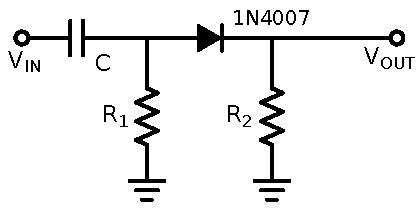
\includegraphics[width=54mm]{schema_peak_detector.pdf}
	\label{fig:schema_peak_detector}
\end{wrapfigure}

Il circuito riportato in Fig. \ref{fig:schema_peak_detector} rappresenta lo schema del rivelatore di fronti d'onda utilizzato il laboratorio. Come vediamo, se si considera solo la parte a monte del diodo, esso risulta un semplice filtro passa alto. Particolarità di tale filtro è il suo utilizzo come derivatore. Infatti, se la capacità $C$ e la resistenza $R_1$ sono piccole vale:

$$ I=\frac{V_{out}'(t)}{R_1}=C\frac{d}{dt}(V_{in}(t)-V_{out}'(t)) \approx C \frac{dV_{in}(t)}{dt} $$

\begin{equation} 
\Rightarrow V_{out}'(t) \approx R_1C \frac{dV_{in}(t)}{dt} 
\label{derivatore}
\end{equation}

L'inserimento del diodo a valle di tale derivatore permette il passaggio dei soli segnali positivi/negativi (in base al verso del diodo stesso).

Per osservare il funzionamento come rivelatore di fronti d'onda abbiamo alimentato il circuito con una forma d'onda quadra di frequenza $100 \si{\hertz}$ e tensione $V_{PP}=10 \si{\volt}$. L'onda quadra ha la particolarità di essere una funzione a tratti. Utilizzando capacità e resistenze molto piccole, il circuito rileverà i punti in cui la derivata tende ad infinito mentre nei tratti in cui la derivata è uguale a zero non lascerà passare nessun segnale (vedi Eq. \ref{derivatore}).

È stata fissata una resistenza $R_2=(1000.4 \pm 0.2) \si{\ohm}$. 

Poichè a parità di segnale in ingresso $V_{in}$ il segnale in uscita dipende sia da $R_1$ che da $C$, abbiamo deciso di effettuare due campionamenti, bloccando una delle due variabili e facendo variare l'altra. Riportiamo nei due seguenti grafici i dati sperimentali da noi ottenuti.

\begin{figure}[h]
\center
	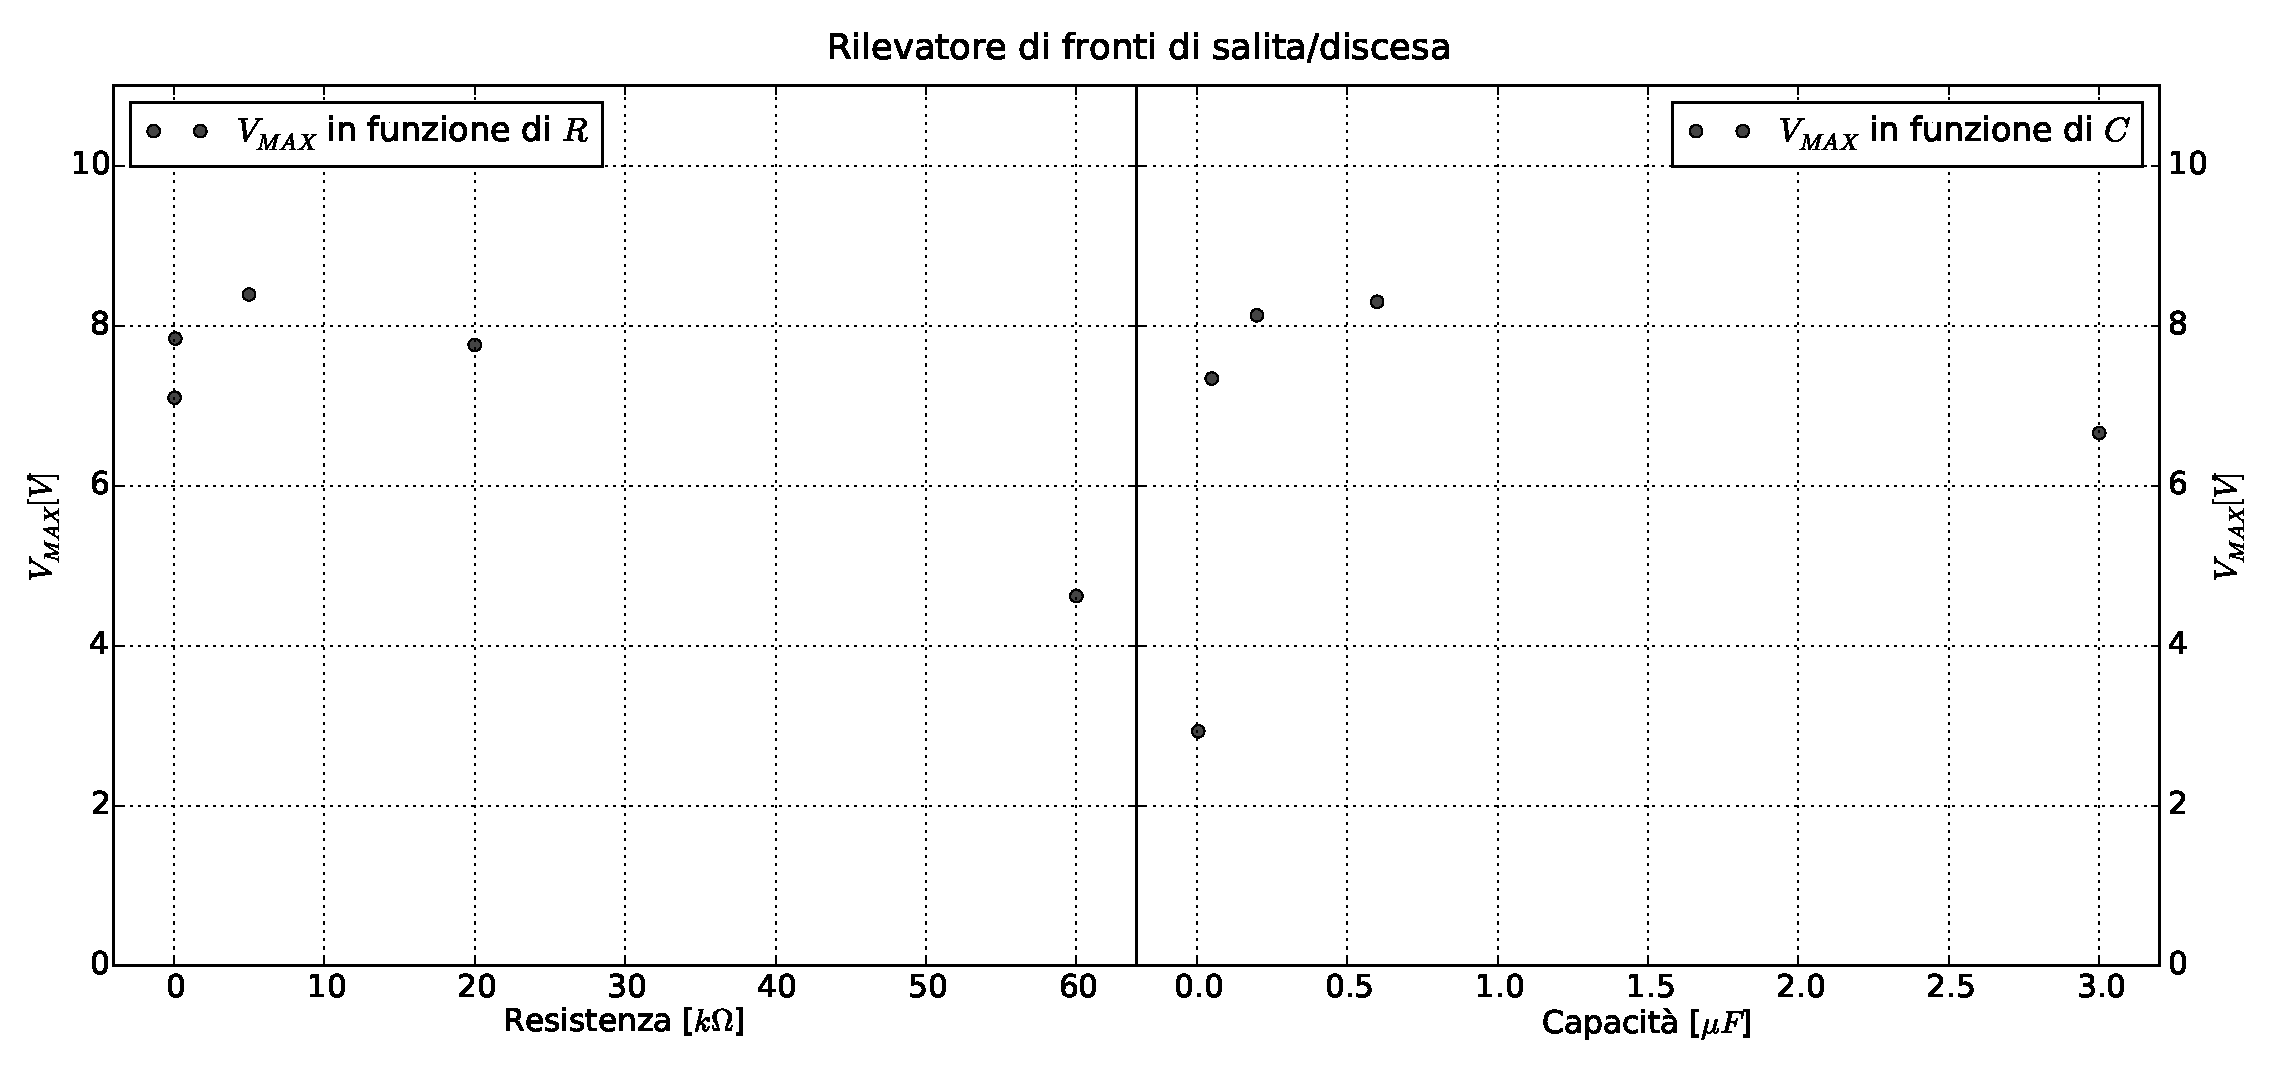
\includegraphics[width=0.75\textwidth]{dati.pdf}
	\caption{Il grafico a sinistra riporta i dati ottenuti variando la resistenza $R$ e tenendo costante la capacità $C = \SI{100}{\nano\farad}$. Nel grafico a destra possiamo invece osservare i valori ottenuti avendo fissato la resistenza $R=\SI{1006}{\ohm}$ e variando la capacità $C$.}
	\label{fig:dati}
\end{figure}


Come vediamo, i valori di tensione $V_{out}^{MAX}$ in entrambi i grafici tendono a valori bassi sia quando valori di resistenza e capacità sono piccoli sia quando sono grandi. Da Eq. (\ref{derivatore}) ci si aspetterebbe che all'aumentare di $R_1$ e $C$ aumenti anche $V_{out}$. Dobbiamo tuttavia ricordare l'approssimazione fatta per ricavare Eq. (\ref{derivatore}). Infatti avevamo assunto che sia capacità che resistenza fossero molto piccole. Evidentemente essa non è più valida per valori troppo grandi di queste due variabili. Ricordiamo anche che sebbene teoricamente l'onda quadra abbia derivata infinita nei punti di discontinuità, non è possibile in laboratorio generare un segnale discontinuo con questa caratteristica. Il valore $\frac{dV_{in}(t)}{dt}=\gamma$  sarà dunque ben definito e potrà essere assunto in prima approssimazione mediamente costante. Per valori piccoli di $C$ ed $R_1$ avremo dunque una legge del tipo $V_{out}^{MAX}= RC \gamma$. \`E dunque evidente che per valori di $R_1\rightarrow 0$ o $C\rightarrow 0$ il valore di tensione in uscita tenderà a zero.
%CONTRADDIZIONE%

Per valori di resistenza e capacità grandi non possiamo fare l'approssimazione di derivatore e dunque non possiamo più ricondurci all'equazione sopra calcolata. Per valori di capacità molto grandi osserveremo una tensione in uscita $V_{out}(t)=I(t) R_1$. Ma $I(t)$ sarà uguale alla corrente di carica/scarica che scorre in un circuito RC. Quando C diventa grande, il condensatore non riuscirà a caricarsi completamente e dunque avremo un valore di tensione $V_{out}$ che decresce aumentando C. Analogamente, quando R diventa molto grande, la corrente che può scorrere nel circuito diventa piccola e dunque il condensatore non riuscirà a caricarsi completamente. Avremo anche in questo caso che la tensione $V_{out}$ decresce aumentando R. Riportiamo per completezza due grafici dei dati visualizzati sull'oscilloscopio. Il primo con $C$ ed $R_1$ piccoli mentre il secondo con $C$ ed $R_1$ abbastanza grandi per apprezzare l'andamento della tensione indotto dalla presenza del condensatore.

\begin{wrapfigure}[19]{r}[0pt]{120mm}
\centering
	\caption{Caratteristica volt-amperometrica del diodo zener BZX85C6V8. I valori di corrente relativi a tensioni comprese tra quelle graficate e l'origine degli assi sono stati esclusi perché poco rilevanti.}
	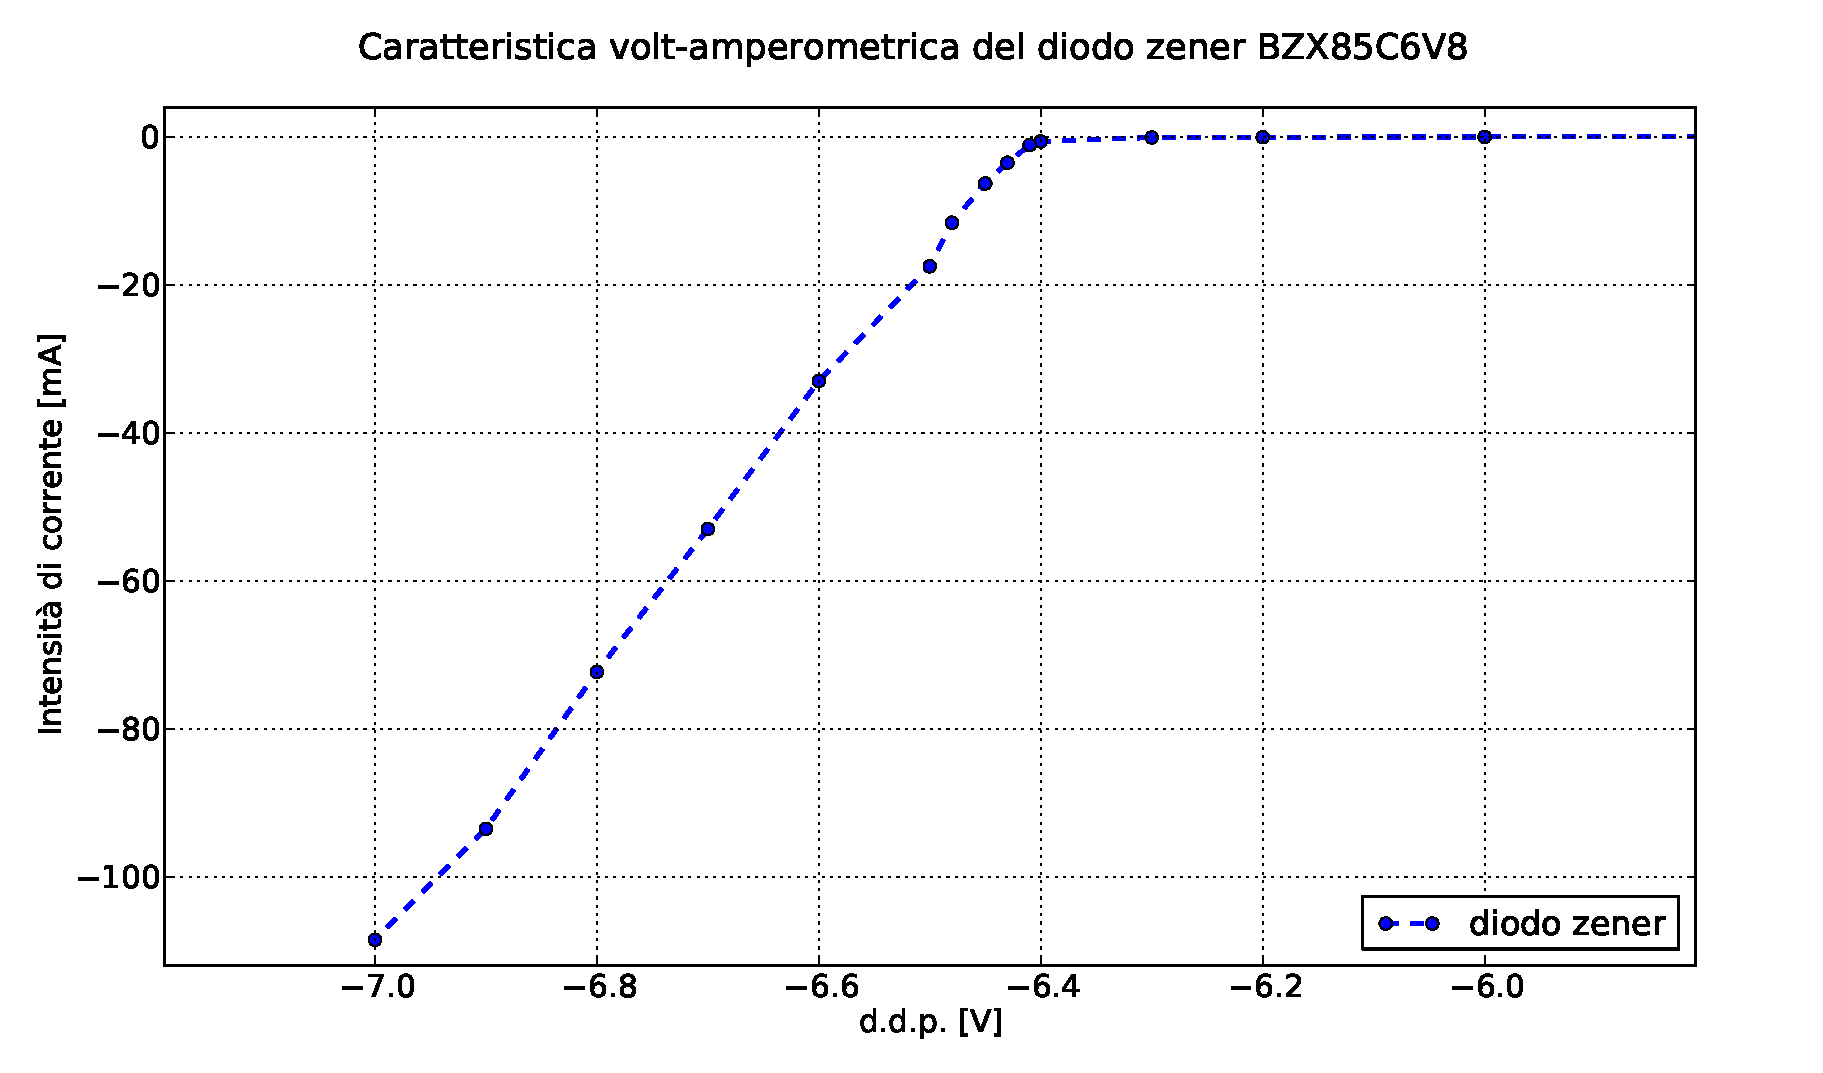
\includegraphics[width=0.55\textwidth]{VI_zener.pdf}
	\label{fig:VI_zener}
\end{wrapfigure}

\begin{figure}[H]
\center
	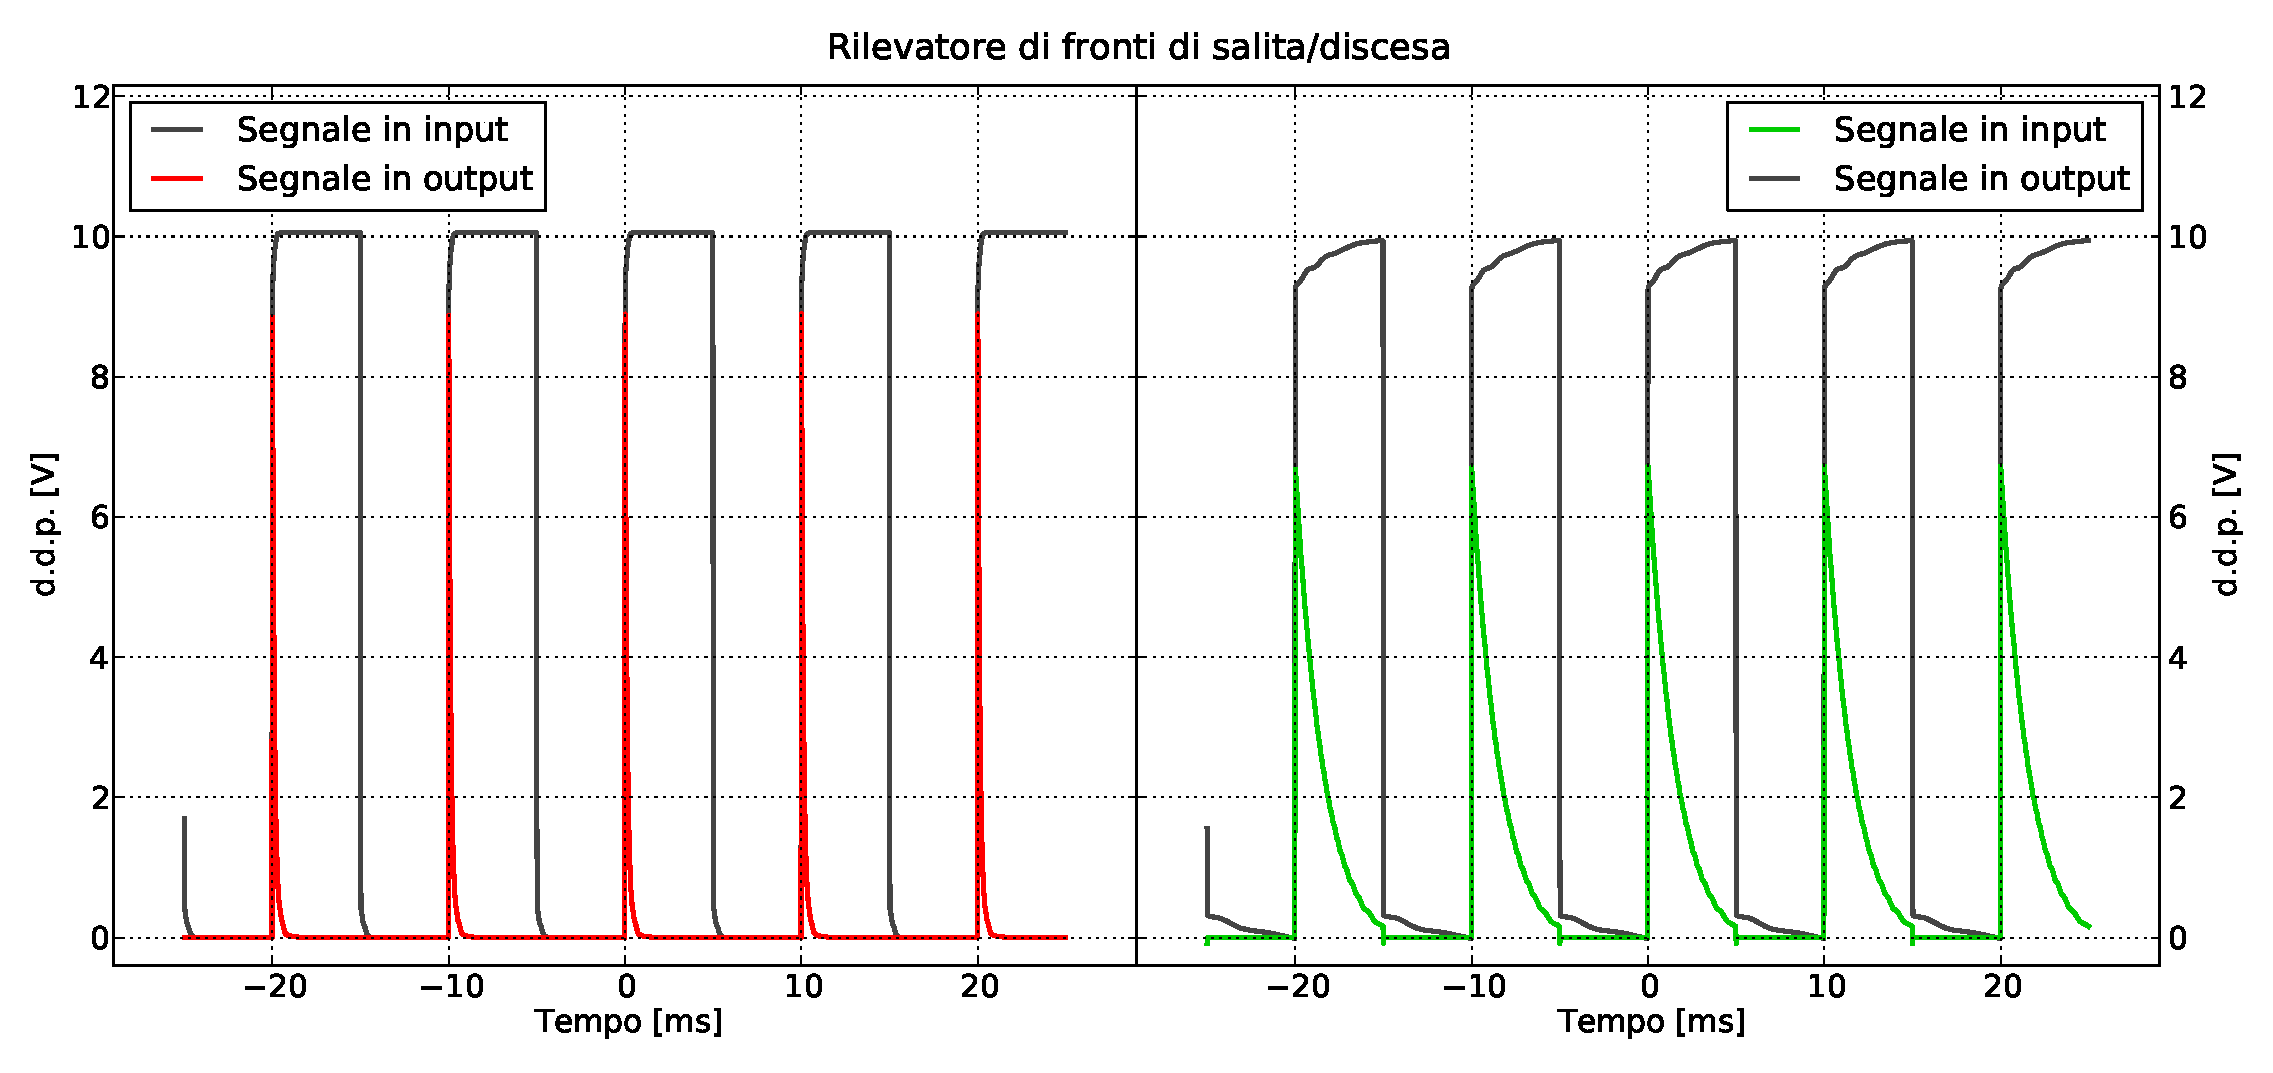
\includegraphics[width=0.80\textwidth]{peaks(2).pdf}
	\caption{Questo doppio grafico riporta le forme d'onda visualizzate a schermo sull'oscilloscopio. Nel grafico a sinistra notiamo il funzionamento del nostro rivelatore di picchi positivi nel range di ``derivatore''. Nel grafico a destra vediamo come la grande capacità del condensatore faccia scorrere nel circuito corrente per più tempo. Notimo inoltre che il generatore di tensione non riesce a fornire sufficiente corrente e dunque l'onda quadra in input risulta distorta.}
	\label{fig:peaks}
\end{figure}

\section{Diodo Zener}

Poichè il diodo zener è pensato per funzionare con polarizzazione inversa, abbiamo campionato solo la caratteristica V-I per valori di tensione negativi. Ricordiamo che a differenza di un diodo come quello utilizzato nell'esperienza precedente, il valore di corrente in funzione della tensione in un diodo zener, una volta raggiunto il range operativo, è lineare. Ovvero esiste una ``resistenza \footnote{Non è possibile chiamarla resistenza in quanto essa è ben definita solo per un insieme ristretto di valori di tensione diverso da tutto l'asse reale.}'', $R_d$, tale che $V=R_d I$.

Utilizzando la breadboard come supporto, abbiamo creato un circuito composto dal generatore di tensione continua (DC $\pm \SI{25}{\volt}$), il diodo zener e il multimetro digitale in modalità amperometro. Aumentando progressivamente la tensione, abbiamo letto sull'amperometro i valori della corrente che attraversava il circuito.
Facendo attenzione che la potenza dissipata dal diodo non superasse quella massima riportata nella scheda tecnica (***********************************), abbiamo campionato l'asse negativo del grafico. Il risultato è esposto in Fig. \ref{fig:VI_zener}.

Dai dati ottenuti è stato possibile calcolare la resistenza dinamica del diodo, ovvero:

\begin{equation}
R_d=\frac{\Delta V}{\Delta I}
\label{scemopagliaccio}
\end{equation}

\begin{wrapfigure}[13]{r}[0pt]{55mm}
	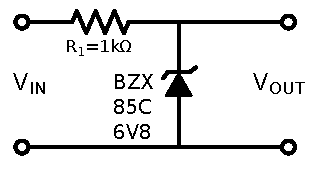
\includegraphics[width=55mm]{schema_zener.pdf}
	\caption{Schema del circuito in cui il diodo Zener BZX85C6V8 è usato come stabilizzatore di tensione.}
	\label{fig:schema_zener}
\end{wrapfigure}

Eseguito un fit lineare\footnote{È immediato verificare che $R_d=\frac{1}{m}$ dove $m$ è la pendenza della retta che interpola i dati oltre la tensione di breakdown.} otteniamo come risultato:
$$R_d= (5.36 \pm 0.06)\,\Omega$$

Il costruttore garantisce una resistenza dinamica $R_d<3.5 \, \Omega$. Ricordiamo che l'amperometro ha una sua resistenza interna e nel nostro caso, avendo impostato il fondoscala a $100mA$, $R_{int}=2\, \Omega$. È dunque immediato calcolare la $R_d$ corretta eseguendo semplicemente la sottrazione delle due. La resistenza dinamica del diodo zener risulta $R_d=3.36 \pm 0.06$.

Nella seconda parte dello studio del diodo zener, abbiamo analizzato il suo funzionamento come stabilizzatore di tensione. Anzitutto è stato montato il circuito riportato in Fig. \ref{fig:schema_zener} con $R = (1000.0 \pm 0.1) \, \si{\ohm}$.  Dallo studio della caratteristica V-I del diodo abbiamo stimato che esso può essere utilizzato come stabilizzatore di tensione da $\SI{-6.5}{\volt}$\footnote{Il costruttore dichiara che la tensione di breakdown è $V_b=6.8 \pm 0.4 V$.} fino a quando la potenza massima dissipata lo permette. 

È stato calcolato il rapporto di stabilizzazione teorico dalla formula (semplice partitore di tensione): 

\begin{equation}
r_{s,teo}\,=\,\frac{R_d}{R+R_d}\,=\, (5.33 \pm 0.06) \times 10^{-3}
\label{RS_teo}
\end{equation}

Riportiamo ora in Fig. \ref{fig:stabilizer} i dati sperimentali da noi ottenuti.

\begin{figure}[h]
\center
	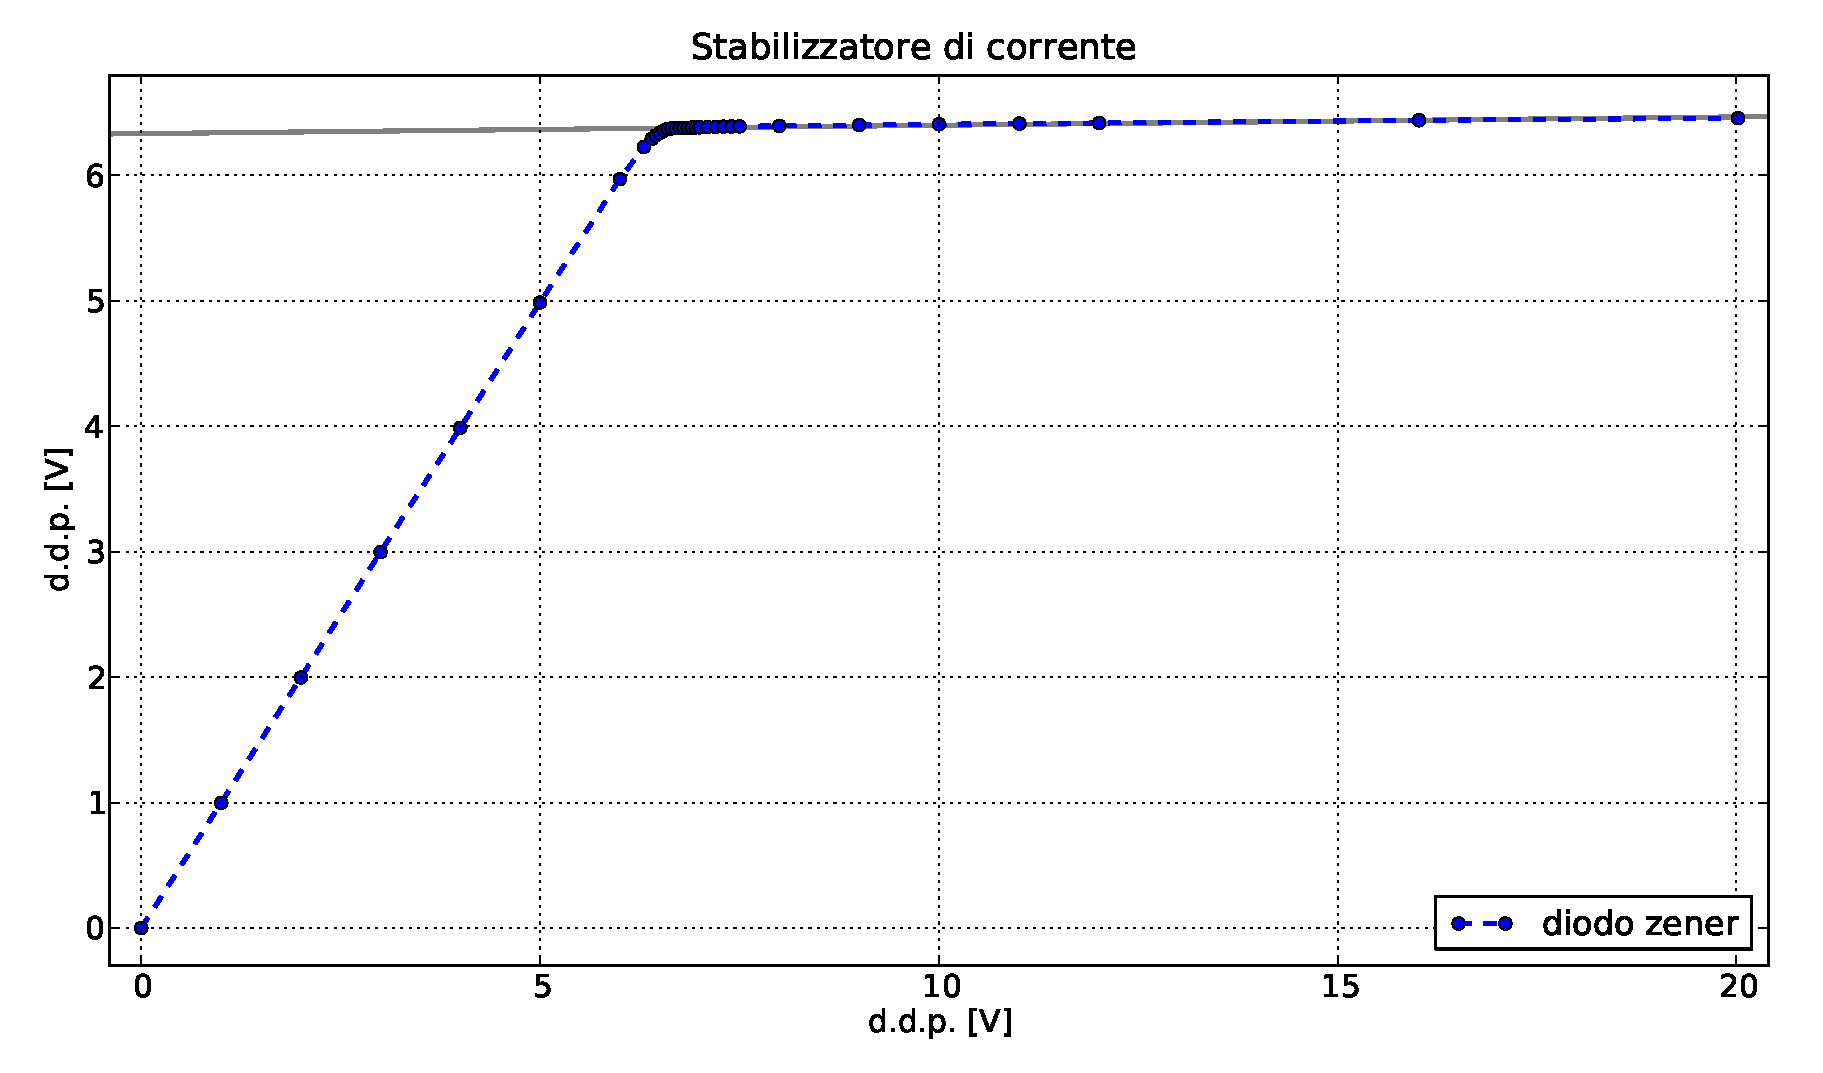
\includegraphics[width=0.66\textwidth]{stabilizer.pdf}
	\caption{Grafico dei dati sperimentali ottenuti per il circuito stabilizzatore di corrente. Come vediamo, uan volta raggiunto il valore di tensione di breakdown, il diodo tende a stabilizzare la tensione del segnale in output al circuito.}
	\label{fig:stabilizer}
\end{figure}

Troviamo ora la pendenza della retta che fitta i dati sperimentali $\frac{\Delta V_{out}}{\Delta V_{in}}$. Tale valore sarà uguale al rapporto di stabilizzazione:

$$r_{s,exp}= (6.6 \pm 0.6) \times 10^{-3} $$

Come si può osservare, i valori teorico e sperimentale del rapporto di stabilizzazione sono compatibli entro un fattore di copertura maggiore o uguale a 2. Riteniamo pertanto che i valori siano coerenti.

Osserviamo infine che il valore del rapporto di stabilizzazione ricavato dalla legge teorica ha una cifra significativa in più del valore ricavato sperimentalmente.